\section{Implementation on a random-access store}
\label{sec:randstore}
A file cannot be allocated as a block of contiguous storage locations, because its length is not
fixed. Neither can it be represented as a linked list of individual elements, because this would
lead to inefficient use of storage - more might be used for the links than the elements themselves.
The solution generally adopted is a compromise between the two extremes: files are represented
as lists of blocks (subsequently called sectors) of fixed length. A block is appended when the last
one is filled. On the average, each file therefore wastes half of a sector. Typical sector sizes are
0.5, 1, 2, or 4 Kbytes, depending on the device used as store.

It immediately follows that access to an element is not as simple as in the case of an array. The
primary concern in the design of a FS and access scheme must be the efficiency of
access to individual elements while scanning the sequence, at least in the case when the next
element lies within the same sector. This access must be no more complicated than a
comparison of two variables followed by an indexed access to the file element and the
incrementing of an address pointing to the element's successor. If the successor lies in another
sector, the procedure may be more involved, as transitions to the next sector occur much less
frequently.

The second most crucial design decision concerns the data structure in which sectors are
organized; it determines how a succeeding sector is located. The simplest solution is to link
sectors in a list. This is acceptable if access is to be restricted to purely sequential scans.
Although this would be sufficient for most applications, it is unnecessarily restrictive for media
other than purely sequential ones (tapes). After all, it is sometimes practical to position a rider at
an arbitrary point in the file rather than always at its beginning. This is made possible by the use
of an indexed sector table, typically stored as a header in the file. The table is an array of the
addresses of the file's data sectors. Unfortunately, the length of the table needed is unknown.
Choosing a fixed length for all files is controversial, because it inevitably leads to either a
limitation of file length (when chosen too small) that is unacceptable in some applications, or to a
large waste of file space (when chosen too large). Experience shows that in practice most files
are quite short, i.e. in the order of a few thousand bytes. The dilemma is avoided by a two-level
table, i.e. by using a table of tables.

The scheme chosen in Oberon is slightly more complex in order to favor short files (< 64 K
bytes): Each file header contains a table of 64 entries, each pointing to a 1K byte sector.
Additionally, it contains a table of 12 entries, the so-called extensions, each pointing to an index
sector containing 256 further sector pointers. The file length is thereby limited to 64 + 12*256
sectors, or 3'211'264 bytes (minus the length of the header). The chosen structure is illustrated in
Fig \ref{fig:file-header}. sec[0] always points to the sector containing the file header.
\begin{figure}
  \label{fig:file-header}
  \centering
  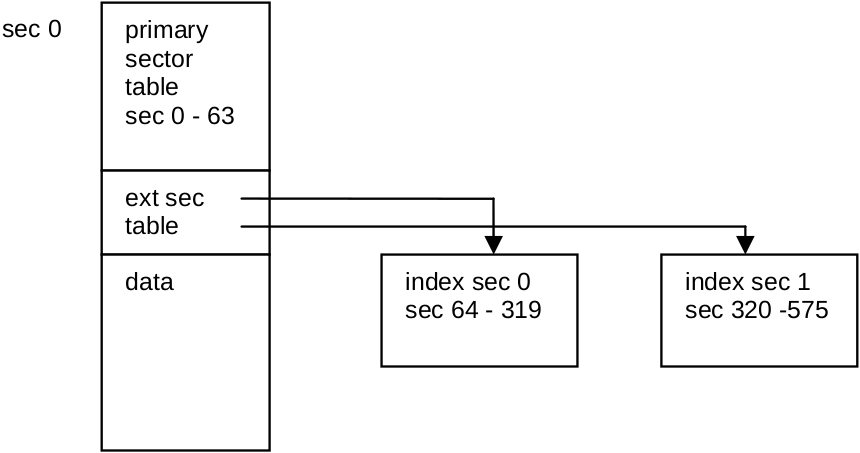
\includegraphics[width=\textwidth]{i/l}
  \caption{File header and extension sectors}
\end{figure}

The header contains some additional data, namely the length of the file (in bytes), its name, and
date and time of its creation. The size of the header is 352 bytes; the remaining 672 bytes of the
first sector are used for data. Hence, truly short files occupy a single sector only. The declaration
of the file header is contained in the definition of module FileDir. An abbreviated version
containing the fields relevant so far is:
\begin{verbatim}
  FileHeader = RECORD
    leng: INT;
    ext: ARRAY 12 OF SectorPointer;
    sec: ARRAY 64 OF SectorPointer
  END
\end{verbatim}

We now turn our attention to the implementation of file access, and first present a system that uses
main storage for the file data instead of a disk and therefore avoids the problems introduced by sector
buffering. The key data structure in this connection is the \verb|Rider|, represented as a record.
\begin{verbatim}
  Rider = RECORD
    eof: BOOL; res, pos, adr: INT;
    file: File
  END
\end{verbatim}

A rider is initialised by a call \verb|Set(r, f, pos)|, which places the rider \verb|r| on file \verb|f|
at position \verb|pos|. From this it is clear that the rider record must contain fields denoting the
attached file and the rider's position on it. We note that they are not exported. However, their values
can be obtained by the function procedures \verb|Pos(r)| and \verb|Base(r)|. This allows a (hidden)
representation most appropriate for an efficient implementation of \verb|Read| and \verb|Write|
without being unsafe.

Consider now the call \verb|Read(r, x)|; its task is to assign the value of the byte designated by the
rider's position to \verb|x| and to advance the position to the next byte. Considering the structure by
which file data are represented, we easily obtain the following program, assuming that the position is
legal, i.e. non-negative and less than the file's length. \verb|a, b, c| are local variables, \verb|HS|
is the size of the header (in sector 0), \verb|SS| is the sector size, typically a power of 2 in order
to make division efficient.
\begin{verbatim}
  a := (r.pos + HS) DIV SS; b := (r.pos + HS) MOD SS;
  IF a < 64 THEN c := r.file.sec[a]
  ELSE c := r.file.ext[(a - 64) DIV 256].sec[(a - 64) MOD 256]
  END ;
  SYSTEM.GET(c + b, x) ; INC (r.pos)
\end{verbatim}

In order to gain efficiency, we use the low-level procedure \verb|GET| that assigns the value at address
\verb|c+b| to \verb|x|. This program is reasonably short, but involves considerable address computations
at every access, and in particular at positions larger than \verb|64 * SS|. Fortunately, there exists an
easy remedy, namely that of caching the address of the current position. This explains the presence of
the field \verb|adr| in the rider record. The resulting program is shown below; note that in order to
avoid the addition of \verb|HS|, \verb|pos| is defined to denote the genuine position, i.e. the abstract
position augmented by \verb|HS|.
\begin{verbatim}
  SYSTEM.GET(r.adr, x); INC(r.adr); INC(r.pos);
  IF r.pos MOD SS = 0 THEN
    m := r.pos DIV SS;
    IF m < 64 THEN r.adr := r.file.sec[m]
    ELSE r.adr := r.file.ext[(m - 64) DIV 256].sec[(m - 64) MOD 256]
    END
  END
\end{verbatim}

We emphasize that in all but one out of 1024 cases only 3 instructions and a single test are to be
executed. This improvement therefore is crucial to the efficiency of file access, and to that of the
entire Oberon. We now present the entire file module (for files on a random-access store).
\begin{verbatim}
MODULE MFiles; (*NW 24.8.90 / 12.10.90 / 20.6.2013*)
  IMPORT SYSTEM, Kernel, FileDir;
  (*A file consists of a sequence of sectors. The first sector contains the header.
    Part of the header is the sector table, an array of addresses to the sectors.
    A file is referenced through riders each of which indicates a position.*)

CONST HS  = FileDir.HeaderSize;
      SS  = FileDir.SectorSize;
      STS = FileDir.SecTabSize;
      XS  = FileDir.IndexSize;

TYPE File* = POINTER TO FileDesc;
     Index = POINTER TO IndexRecord;
     IndexRecord = RECORD sec: FileDir.IndexSector END ;
     Rider*      = RECORD eof*: BOOL;
       res*, pos, adr: INT;
       file: File
     END ;
     FileDesc    = RECORD mark: INT;
       name: FileDir.FileName;
       len, date: INT;
       ext: ARRAY FileDir.ExTabSize OF Index;
       sec: FileDir.SectorTable
     END ;

PROC Old*(name: ARRAY OF CHAR): File;
  VAR head: INT;
   namebuf: FileDir.FileName;
BEGIN
  FileDir.Search(name, head); RETURN SYSTEM.VAL(File, head)
END Old;

PROC New*(name: ARRAY OF CHAR): File;
  VAR f: File; head: INT;
BEGIN f := NIL; Kernel.AllocSector(0, head);
  IF head # 0 THEN
  f := SYSTEM.VAL(File, head); f.mark := FileDir.HeaderMark;
  f.len := HS; f.name := name;
  f.date := Kernel.Clock(); f.sec[0] := head
  END ;
  RETURN f
END New;

PROC Register*(f: File);
BEGIN
  IF (f # NIL) & (f.name[0] > 0X) THEN FileDir.Insert(f.name, f.sec[0]) END ;
END Register;

PROC Length*(f: File): INT;
BEGIN RETURN f.len - HS
END Length;

PROC Date*(f: File): INT;
BEGIN RETURN f.date
END Date;

PROC Set*(VAR r: Rider; f: File; pos: LONGINT);
  VAR m, n: INT;
BEGIN r.eof := FALSE; r.res := 0;
  IF f # NIL THEN
    IF pos < 0 THEN r.pos := HS
    ELSIF pos > f.len - HS THEN r.pos := f.len
    ELSE r.pos := pos + HS
    END ;
    r.file := f; m := r.pos DIV SS; n := r.pos MOD SS;
    IF m < STS THEN r.adr := f.sec[m] + n
    ELSE r.adr := f.ext[(m-STS) DIV XS].sec[(m-STS) MOD XS] + n
    END
  END
END Set;

PROC ReadByte*(VAR r: Rider; VAR x: BYTE);
  VAR m: INT;
BEGIN
  IF r.pos < r.file.len THEN
    SYSTEM.GET(r.adr, x); INC(r.adr); INC(r.pos);
    IF r.adr MOD SS = 0 THEN
      m := r.pos DIV SS;
      IF m < STS THEN r.adr := r.file.sec[m]
      ELSE r.adr := r.file.ext[(m-STS) DIV XS].sec[(m-STS) MOD XS]
      END
    END
  ELSE x := 0; r.eof := TRUE
  END
END ReadByte;

PROC WriteByte*(VAR r: Rider; x: BYTE);
  VAR k, m, n, ix: INT;
BEGIN
  IF r.pos < r.file.len THEN
    m := r.pos DIV SS; INC(r.pos);
    IF m < STS THEN r.adr := r.file.sec[m]
    ELSE r.adr := r.file.ext[(m-STS) DIV XS].sec[(m-STS) MOD XS]
    END
  ELSE
    IF r.adr MOD SS = 0 THEN
      m := r.pos DIV SS;
      IF m < STS THEN Kernel.AllocSector(0, r.adr); r.file.sec[m] := r.adr
      ELSE n := (m - STS) DIV XS; k := (m - STS) MOD XS;
        IF k = 0 THEN (*new index*)
          Kernel.AllocSector(0, ix); r.file.ext[n] := SYSTEM.VAL(Index, ix)
        END ;
        Kernel.AllocSector(0, r.adr); r.file.ext[n].sec[k] := r.adr
      END
    END ;
    INC(r.pos); r.file.len := r.pos
  END ;
  SYSTEM.PUT(r.adr, x); INC(r.adr)
END WriteByte;

PROC Pos*(VAR r: Rider): INT;
BEGIN RETURN r.pos - HS
END Pos;

PROC Base*(VAR r: Rider): File;
BEGIN RETURN r.file
END Base;

END MFiles.
\end{verbatim}

Allocation of a new sector occurs upon creating a file (\verb|Files.New|), and when writing at the end
of a file after the current sector had been filled. Procedure \verb|AllocSector| yields the address of
the allocated sector. It is determined by a search in the sector reservation table for a free sector. In
this table, every sector is represented by a single bit indicating whether or not the sector is
allocated. Although conceptually belonging to the FS, this table resides within module \verb|Kernel|.

Deallocation of a file's sectors could occur as soon as the file is no longer accessible, neither
through a variable of any loaded module nor from the file directory. However, this moment is
difficult to determine. Therefore, the method of garbage collection is used in Oberon for the
deallocation of file space. In consideration of the fact that file space is large and the collection of
unused sectors relatively time-consuming, we confine this process to system initialization. It is
represented by procedure \verb|FileDir.Init|. At that time, the only referenced files are those
registered in the directory. Init therefore scans the entire directory and records the sectors
referenced in each file in the sector reservation table (see \S \ref{sec:dir}).

For applications where system startup and initialization is supposed to occur very infrequently, such as
for server systems, a procedure \verb|Files.Purge| is provided. Its effect is to return the sectors used
by the specified file to the pool of free sectors. Evidently, the programmer then bears the
responsibility to guarantee that no references to the purged file continue to exist. This may be
possible in a closed server system, but files should not be purged under normal circumstances, as a
violation of said precondition will lead to unpredictable disaster.  The following procedures used for
allocating, deallocating, and marking sectors in the sector reservation table
are defined in module \verb|Kernel|:
\begin{verbatim}
  PROC AllocSector(hint: INT; VAR sec: INT); (*used in WriteByte*)
  PROC MarkSector(sec: INT);                 (*used in Init*)
  PROC FreeSector(sec: INT);                 (*used in Purge*)
\end{verbatim}
